%%%%%%%%%%%%%%%%%%%%%%% file template.tex %%%%%%%%%%%%%%%%%%%%%%%%%
%
% This is a general template file for the LaTeX package SVJour3
% for Springer journals.          Springer Heidelberg 2010/09/16
%
% Copy it to a new file with a new name and use it as the basis
% for your article. Delete % signs as needed.
%
% This template includes a few options for different layouts and
% content for various journals. Please consult a previous issue of
% your journal as needed.
%
%%%%%%%%%%%%%%%%%%%%%%%%%%%%%%%%%%%%%%%%%%%%%%%%%%%%%%%%%%%%%%%%%%%
%
% First comes an example EPS file -- just ignore it and
% proceed on the \documentclass line
% your LaTeX will extract the file if required
% \begin{filecontents*}{example.eps}
% %!PS-Adobe-3.0 EPSF-3.0
% %%BoundingBox: 19 19 221 221
% %%CreationDate: Mon Sep 29 1997
% %%Creator: programmed by hand (JK)
% %%EndComments
% gsave
% newpath
%   20 20 moveto
%   20 220 lineto
%   220 220 lineto
%   220 20 lineto
% closepath
% 2 setlinewidth
% gsave
%   .4 setgray fill
% grestore
% stroke
% grestore
% \end{filecontents*}
%
\RequirePackage{fix-cm}
%
%\documentclass{svjour3}                     % onecolumn (standard format)
%\documentclass[smallcondensed]{svjour3}     % onecolumn (ditto)
\documentclass[smallextended]{svjour3}    
% onecolumn (second format)
%\documentclass[twocolumn]{svjour3}          % twocolumn
%
\smartqed  % flush right qed marks, e.g. at end of proof
%
\usepackage{adjustbox}
\usepackage{multirow}
\usepackage{appendix}
\usepackage{booktabs,caption}
\usepackage[flushleft]{threeparttable}
\usepackage{orcidlink}
\usepackage{comment}
\usepackage {drafts}
\usepackage{subfigure}
\usepackage{listings}
\usepackage{courier}
\usepackage{array}
\usepackage{longtable}
\usepackage{circledsteps}
\usepackage{float}

\usepackage{xurl} 


\usepackage{cite}
\usepackage{amsmath,amssymb,amsfonts}
\usepackage{algorithmic}
\usepackage{graphicx}
\usepackage{textcomp}
\usepackage{xcolor}
\usepackage{url}
\usepackage[nolist]{acronym}% consistently use acronyms
%%%%%%%%%%%---SETME-----%%%%%%%%%%%%%
%replace @@ with the submission number submission site.
\newcommand{\thiswork}{INF$^2$\xspace}
%%%%%%%%%%%%%%%%%%%%%%%%%%%%%%%%%%%%


%\newcommand{\rev}[1]{{\color{olivegreen}#1}}
\newcommand{\rev}[1]{{#1}}


\newcommand{\JL}[1]{{\color{cyan}[\textbf{\sc JLee}: \textit{#1}]}}
\newcommand{\JW}[1]{{\color{orange}[\textbf{\sc JJung}: \textit{#1}]}}
\newcommand{\JY}[1]{{\color{blue(ncs)}[\textbf{\sc JSong}: \textit{#1}]}}
\newcommand{\HS}[1]{{\color{magenta}[\textbf{\sc HJang}: \textit{#1}]}}
\newcommand{\CS}[1]{{\color{navy}[\textbf{\sc CShin}: \textit{#1}]}}
\newcommand{\SN}[1]{{\color{olive}[\textbf{\sc SNoh}: \textit{#1}]}}

%\def\final{}   % uncomment this for the submission version
\ifdefined\final
\renewcommand{\JL}[1]{}
\renewcommand{\JW}[1]{}
\renewcommand{\JY}[1]{}
\renewcommand{\HS}[1]{}
\renewcommand{\CS}[1]{}
\renewcommand{\SN}[1]{}
\fi

%%% Notion for baseline approaches %%% 
\newcommand{\baseline}{offloading-based batched inference\xspace}
\newcommand{\Baseline}{Offloading-based batched inference\xspace}


\newcommand{\ans}{attention-near storage\xspace}
\newcommand{\Ans}{Attention-near storage\xspace}
\newcommand{\ANS}{Attention-Near Storage\xspace}

\newcommand{\wb}{delayed KV cache writeback\xspace}
\newcommand{\Wb}{Delayed KV cache writeback\xspace}
\newcommand{\WB}{Delayed KV Cache Writeback\xspace}

\newcommand{\xcache}{X-cache\xspace}
\newcommand{\XCACHE}{X-Cache\xspace}


%%% Notions for our methods %%%
\newcommand{\schemea}{\textbf{Expanding supported maximum sequence length with optimized performance}\xspace}
\newcommand{\Schemea}{\textbf{Expanding supported maximum sequence length with optimized performance}\xspace}

\newcommand{\schemeb}{\textbf{Optimizing the storage device performance}\xspace}
\newcommand{\Schemeb}{\textbf{Optimizing the storage device performance}\xspace}

\newcommand{\schemec}{\textbf{Orthogonally supporting Compression Techniques}\xspace}
\newcommand{\Schemec}{\textbf{Orthogonally supporting Compression Techniques}\xspace}



% Circular numbers
\usepackage{tikz}
\newcommand*\circled[1]{\tikz[baseline=(char.base)]{
            \node[shape=circle,draw,inner sep=0.4pt] (char) {#1};}}

\newcommand*\bcircled[1]{\tikz[baseline=(char.base)]{
            \node[shape=circle,draw,inner sep=0.4pt, fill=black, text=white] (char) {#1};}}
\def\BibTeX{{\rm B\kern-.05em{\sc i\kern-.025em b}\kern-.08em
    T\kern-.1667em\lower.7ex\hbox{E}\kern-.125emX}}
%
% \usepackage{mathptmx}      % use Times fonts if available on your TeX system
%
% insert here the call for the packages your document requires
%\usepackage{latexsym}
% etc.
%
% please place your own definitions here and don't use \def but
% \newcommand{}{}
%
% Insert the name of "your journal" with
% \journalname{myjournal}
%
\begin{document}



\title{Modeling in \jjodel: Bridging Complexity and Usability in Model-Driven Engineering}
%\subtitle{Do you have a subtitle?\\ If so, write it here}

\titlerunning{Modeling in \jjodel{}}        % if too long for running head

\author{Antonio Bucchiarone \orcidlink{0000-0003-1154-1382}        \and
        Juri Di Rocco\orcidlink{0000-0002-7909-3902}     \and 
        Damiano Di Vincenzo \and
        Alfonso Pierantonio  \orcidlink{0000-0002-5231-3952} 
}


\institute{SWEN, Università degli Studi dell'Aquila, 67100, L'Aquila, Italy\\ \email{\{name.surname\}@univaq.it}\\ \email{damiano.divincenzo@studenti.univaq.it}
}

\authorrunning{A. Bucchiarone et al.} % if too long for running head

 

\date{Received: date / Accepted: date}
% The correct dates will be entered by the editor


\maketitle
\begin{abstract}

\jjodel{} is a cloud-based reflective platform designed to address the challenges of Model-Driven Engineering (MDE), particularly the cognitive complexity and usability barriers often encountered in existing model-driven tools. This article presents the motivation and requirements behind the design of \jjodel{} and demonstrates how it satisfies these through its key features. By offering a low-code environment with modular viewpoints for syntax, validation, and semantics, \jjodel{} empowers language designers to define and refine domain-specific languages (DSLs) with ease. Its innovative capabilities, such as real-time collaboration, live co-evolution support, and syntax customization, ensure adaptability and scalability for academic and industrial contexts. A practical case study of an algebraic expression language highlights the ability of \jjodel{} to manage positional semantics and event-driven workflows, illustrating its effectiveness in simplifying complex modeling scenarios. Built on modern front-end technologies, \jjodel{} bridges the gap between theoretical MDE research and practical application, providing a versatile and accessible solution for diverse modeling needs.

\end{abstract}

\keywords{Model-Driven Engineering (MDE) \and reflective platforms \and low-code development \and \jjodel{} \and collaborative modeling \and co-evolution}

\section{Introduction}\label{sec1}
\section{Introduction}
\label{sec:introduction}
The business processes of organizations are experiencing ever-increasing complexity due to the large amount of data, high number of users, and high-tech devices involved \cite{martin2021pmopportunitieschallenges, beerepoot2023biggestbpmproblems}. This complexity may cause business processes to deviate from normal control flow due to unforeseen and disruptive anomalies \cite{adams2023proceddsriftdetection}. These control-flow anomalies manifest as unknown, skipped, and wrongly-ordered activities in the traces of event logs monitored from the execution of business processes \cite{ko2023adsystematicreview}. For the sake of clarity, let us consider an illustrative example of such anomalies. Figure \ref{FP_ANOMALIES} shows a so-called event log footprint, which captures the control flow relations of four activities of a hypothetical event log. In particular, this footprint captures the control-flow relations between activities \texttt{a}, \texttt{b}, \texttt{c} and \texttt{d}. These are the causal ($\rightarrow$) relation, concurrent ($\parallel$) relation, and other ($\#$) relations such as exclusivity or non-local dependency \cite{aalst2022pmhandbook}. In addition, on the right are six traces, of which five exhibit skipped, wrongly-ordered and unknown control-flow anomalies. For example, $\langle$\texttt{a b d}$\rangle$ has a skipped activity, which is \texttt{c}. Because of this skipped activity, the control-flow relation \texttt{b}$\,\#\,$\texttt{d} is violated, since \texttt{d} directly follows \texttt{b} in the anomalous trace.
\begin{figure}[!t]
\centering
\includegraphics[width=0.9\columnwidth]{images/FP_ANOMALIES.png}
\caption{An example event log footprint with six traces, of which five exhibit control-flow anomalies.}
\label{FP_ANOMALIES}
\end{figure}

\subsection{Control-flow anomaly detection}
Control-flow anomaly detection techniques aim to characterize the normal control flow from event logs and verify whether these deviations occur in new event logs \cite{ko2023adsystematicreview}. To develop control-flow anomaly detection techniques, \revision{process mining} has seen widespread adoption owing to process discovery and \revision{conformance checking}. On the one hand, process discovery is a set of algorithms that encode control-flow relations as a set of model elements and constraints according to a given modeling formalism \cite{aalst2022pmhandbook}; hereafter, we refer to the Petri net, a widespread modeling formalism. On the other hand, \revision{conformance checking} is an explainable set of algorithms that allows linking any deviations with the reference Petri net and providing the fitness measure, namely a measure of how much the Petri net fits the new event log \cite{aalst2022pmhandbook}. Many control-flow anomaly detection techniques based on \revision{conformance checking} (hereafter, \revision{conformance checking}-based techniques) use the fitness measure to determine whether an event log is anomalous \cite{bezerra2009pmad, bezerra2013adlogspais, myers2018icsadpm, pecchia2020applicationfailuresanalysispm}. 

The scientific literature also includes many \revision{conformance checking}-independent techniques for control-flow anomaly detection that combine specific types of trace encodings with machine/deep learning \cite{ko2023adsystematicreview, tavares2023pmtraceencoding}. Whereas these techniques are very effective, their explainability is challenging due to both the type of trace encoding employed and the machine/deep learning model used \cite{rawal2022trustworthyaiadvances,li2023explainablead}. Hence, in the following, we focus on the shortcomings of \revision{conformance checking}-based techniques to investigate whether it is possible to support the development of competitive control-flow anomaly detection techniques while maintaining the explainable nature of \revision{conformance checking}.
\begin{figure}[!t]
\centering
\includegraphics[width=\columnwidth]{images/HIGH_LEVEL_VIEW.png}
\caption{A high-level view of the proposed framework for combining \revision{process mining}-based feature extraction with dimensionality reduction for control-flow anomaly detection.}
\label{HIGH_LEVEL_VIEW}
\end{figure}

\subsection{Shortcomings of \revision{conformance checking}-based techniques}
Unfortunately, the detection effectiveness of \revision{conformance checking}-based techniques is affected by noisy data and low-quality Petri nets, which may be due to human errors in the modeling process or representational bias of process discovery algorithms \cite{bezerra2013adlogspais, pecchia2020applicationfailuresanalysispm, aalst2016pm}. Specifically, on the one hand, noisy data may introduce infrequent and deceptive control-flow relations that may result in inconsistent fitness measures, whereas, on the other hand, checking event logs against a low-quality Petri net could lead to an unreliable distribution of fitness measures. Nonetheless, such Petri nets can still be used as references to obtain insightful information for \revision{process mining}-based feature extraction, supporting the development of competitive and explainable \revision{conformance checking}-based techniques for control-flow anomaly detection despite the problems above. For example, a few works outline that token-based \revision{conformance checking} can be used for \revision{process mining}-based feature extraction to build tabular data and develop effective \revision{conformance checking}-based techniques for control-flow anomaly detection \cite{singh2022lapmsh, debenedictis2023dtadiiot}. However, to the best of our knowledge, the scientific literature lacks a structured proposal for \revision{process mining}-based feature extraction using the state-of-the-art \revision{conformance checking} variant, namely alignment-based \revision{conformance checking}.

\subsection{Contributions}
We propose a novel \revision{process mining}-based feature extraction approach with alignment-based \revision{conformance checking}. This variant aligns the deviating control flow with a reference Petri net; the resulting alignment can be inspected to extract additional statistics such as the number of times a given activity caused mismatches \cite{aalst2022pmhandbook}. We integrate this approach into a flexible and explainable framework for developing techniques for control-flow anomaly detection. The framework combines \revision{process mining}-based feature extraction and dimensionality reduction to handle high-dimensional feature sets, achieve detection effectiveness, and support explainability. Notably, in addition to our proposed \revision{process mining}-based feature extraction approach, the framework allows employing other approaches, enabling a fair comparison of multiple \revision{conformance checking}-based and \revision{conformance checking}-independent techniques for control-flow anomaly detection. Figure \ref{HIGH_LEVEL_VIEW} shows a high-level view of the framework. Business processes are monitored, and event logs obtained from the database of information systems. Subsequently, \revision{process mining}-based feature extraction is applied to these event logs and tabular data input to dimensionality reduction to identify control-flow anomalies. We apply several \revision{conformance checking}-based and \revision{conformance checking}-independent framework techniques to publicly available datasets, simulated data of a case study from railways, and real-world data of a case study from healthcare. We show that the framework techniques implementing our approach outperform the baseline \revision{conformance checking}-based techniques while maintaining the explainable nature of \revision{conformance checking}.

In summary, the contributions of this paper are as follows.
\begin{itemize}
    \item{
        A novel \revision{process mining}-based feature extraction approach to support the development of competitive and explainable \revision{conformance checking}-based techniques for control-flow anomaly detection.
    }
    \item{
        A flexible and explainable framework for developing techniques for control-flow anomaly detection using \revision{process mining}-based feature extraction and dimensionality reduction.
    }
    \item{
        Application to synthetic and real-world datasets of several \revision{conformance checking}-based and \revision{conformance checking}-independent framework techniques, evaluating their detection effectiveness and explainability.
    }
\end{itemize}

The rest of the paper is organized as follows.
\begin{itemize}
    \item Section \ref{sec:related_work} reviews the existing techniques for control-flow anomaly detection, categorizing them into \revision{conformance checking}-based and \revision{conformance checking}-independent techniques.
    \item Section \ref{sec:abccfe} provides the preliminaries of \revision{process mining} to establish the notation used throughout the paper, and delves into the details of the proposed \revision{process mining}-based feature extraction approach with alignment-based \revision{conformance checking}.
    \item Section \ref{sec:framework} describes the framework for developing \revision{conformance checking}-based and \revision{conformance checking}-independent techniques for control-flow anomaly detection that combine \revision{process mining}-based feature extraction and dimensionality reduction.
    \item Section \ref{sec:evaluation} presents the experiments conducted with multiple framework and baseline techniques using data from publicly available datasets and case studies.
    \item Section \ref{sec:conclusions} draws the conclusions and presents future work.
\end{itemize}

\section{Overview of \jjodel{}}
\label{sec:overview}
\section{Overview}

\revision{In this section, we first explain the foundational concept of Hausdorff distance-based penetration depth algorithms, which are essential for understanding our method (Sec.~\ref{sec:preliminary}).
We then provide a brief overview of our proposed RT-based penetration depth algorithm (Sec.~\ref{subsec:algo_overview}).}



\section{Preliminaries }
\label{sec:Preliminaries}

% Before we introduce our method, we first overview the important basics of 3D dynamic human modeling with Gaussian splatting. Then, we discuss the diffusion-based 3d generation techniques, and how they can be applied to human modeling.
% \ZY{I stopp here. TBC.}
% \subsection{Dynamic human modeling with Gaussian splatting}
\subsection{3D Gaussian Splatting}
3D Gaussian splatting~\cite{kerbl3Dgaussians} is an explicit scene representation that allows high-quality real-time rendering. The given scene is represented by a set of static 3D Gaussians, which are parameterized as follows: Gaussian center $x\in {\mathbb{R}^3}$, color $c\in {\mathbb{R}^3}$, opacity $\alpha\in {\mathbb{R}}$, spatial rotation in the form of quaternion $q\in {\mathbb{R}^4}$, and scaling factor $s\in {\mathbb{R}^3}$. Given these properties, the rendering process is represented as:
\begin{equation}
  I = Splatting(x, c, s, \alpha, q, r),
  \label{eq:splattingGA}
\end{equation}
where $I$ is the rendered image, $r$ is a set of query rays crossing the scene, and $Splatting(\cdot)$ is a differentiable rendering process. We refer readers to Kerbl et al.'s paper~\cite{kerbl3Dgaussians} for the details of Gaussian splatting. 



% \ZY{I would suggest move this part to the method part.}
% GaissianAvatar is a dynamic human generation model based on Gaussian splitting. Given a sequence of RGB images, this method utilizes fitted SMPLs and sampled points on its surface to obtain a pose-dependent feature map by a pose encoder. The pose-dependent features and a geometry feature are fed in a Gaussian decoder, which is employed to establish a functional mapping from the underlying geometry of the human form to diverse attributes of 3D Gaussians on the canonical surfaces. The parameter prediction process is articulated as follows:
% \begin{equation}
%   (\Delta x,c,s)=G_{\theta}(S+P),
%   \label{eq:gaussiandecoder}
% \end{equation}
%  where $G_{\theta}$ represents the Gaussian decoder, and $(S+P)$ is the multiplication of geometry feature S and pose feature P. Instead of optimizing all attributes of Gaussian, this decoder predicts 3D positional offset $\Delta{x} \in {\mathbb{R}^3}$, color $c\in\mathbb{R}^3$, and 3D scaling factor $ s\in\mathbb{R}^3$. To enhance geometry reconstruction accuracy, the opacity $\alpha$ and 3D rotation $q$ are set to fixed values of $1$ and $(1,0,0,0)$ respectively.
 
%  To render the canonical avatar in observation space, we seamlessly combine the Linear Blend Skinning function with the Gaussian Splatting~\cite{kerbl3Dgaussians} rendering process: 
% \begin{equation}
%   I_{\theta}=Splatting(x_o,Q,d),
%   \label{eq:splatting}
% \end{equation}
% \begin{equation}
%   x_o = T_{lbs}(x_c,p,w),
%   \label{eq:LBS}
% \end{equation}
% where $I_{\theta}$ represents the final rendered image, and the canonical Gaussian position $x_c$ is the sum of the initial position $x$ and the predicted offset $\Delta x$. The LBS function $T_{lbs}$ applies the SMPL skeleton pose $p$ and blending weights $w$ to deform $x_c$ into observation space as $x_o$. $Q$ denotes the remaining attributes of the Gaussians. With the rendering process, they can now reposition these canonical 3D Gaussians into the observation space.



\subsection{Score Distillation Sampling}
Score Distillation Sampling (SDS)~\cite{poole2022dreamfusion} builds a bridge between diffusion models and 3D representations. In SDS, the noised input is denoised in one time-step, and the difference between added noise and predicted noise is considered SDS loss, expressed as:

% \begin{equation}
%   \mathcal{L}_{SDS}(I_{\Phi}) \triangleq E_{t,\epsilon}[w(t)(\epsilon_{\phi}(z_t,y,t)-\epsilon)\frac{\partial I_{\Phi}}{\partial\Phi}],
%   \label{eq:SDSObserv}
% \end{equation}
\begin{equation}
    \mathcal{L}_{\text{SDS}}(I_{\Phi}) \triangleq \mathbb{E}_{t,\epsilon} \left[ w(t) \left( \epsilon_{\phi}(z_t, y, t) - \epsilon \right) \frac{\partial I_{\Phi}}{\partial \Phi} \right],
  \label{eq:SDSObservGA}
\end{equation}
where the input $I_{\Phi}$ represents a rendered image from a 3D representation, such as 3D Gaussians, with optimizable parameters $\Phi$. $\epsilon_{\phi}$ corresponds to the predicted noise of diffusion networks, which is produced by incorporating the noise image $z_t$ as input and conditioning it with a text or image $y$ at timestep $t$. The noise image $z_t$ is derived by introducing noise $\epsilon$ into $I_{\Phi}$ at timestep $t$. The loss is weighted by the diffusion scheduler $w(t)$. 
% \vspace{-3mm}

\subsection{Overview of the RTPD Algorithm}\label{subsec:algo_overview}
Fig.~\ref{fig:Overview} presents an overview of our RTPD algorithm.
It is grounded in the Hausdorff distance-based penetration depth calculation method (Sec.~\ref{sec:preliminary}).
%, similar to that of Tang et al.~\shortcite{SIG09HIST}.
The process consists of two primary phases: penetration surface extraction and Hausdorff distance calculation.
We leverage the RTX platform's capabilities to accelerate both of these steps.

\begin{figure*}[t]
    \centering
    \includegraphics[width=0.8\textwidth]{Image/overview.pdf}
    \caption{The overview of RT-based penetration depth calculation algorithm overview}
    \label{fig:Overview}
\end{figure*}

The penetration surface extraction phase focuses on identifying the overlapped region between two objects.
\revision{The penetration surface is defined as a set of polygons from one object, where at least one of its vertices lies within the other object. 
Note that in our work, we focus on triangles rather than general polygons, as they are processed most efficiently on the RTX platform.}
To facilitate this extraction, we introduce a ray-tracing-based \revision{Point-in-Polyhedron} test (RT-PIP), significantly accelerated through the use of RT cores (Sec.~\ref{sec:RT-PIP}).
This test capitalizes on the ray-surface intersection capabilities of the RTX platform.
%
Initially, a Geometry Acceleration Structure (GAS) is generated for each object, as required by the RTX platform.
The RT-PIP module takes the GAS of one object (e.g., $GAS_{A}$) and the point set of the other object (e.g., $P_{B}$).
It outputs a set of points (e.g., $P_{\partial B}$) representing the penetration region, indicating their location inside the opposing object.
Subsequently, a penetration surface (e.g., $\partial B$) is constructed using this point set (e.g., $P_{\partial B}$) (Sec.~\ref{subsec:surfaceGen}).
%
The generated penetration surfaces (e.g., $\partial A$ and $\partial B$) are then forwarded to the next step. 

The Hausdorff distance calculation phase utilizes the ray-surface intersection test of the RTX platform (Sec.~\ref{sec:RT-Hausdorff}) to compute the Hausdorff distance between two objects.
We introduce a novel Ray-Tracing-based Hausdorff DISTance algorithm, RT-HDIST.
It begins by generating GAS for the two penetration surfaces, $P_{\partial A}$ and $P_{\partial B}$, derived from the preceding step.
RT-HDIST processes the GAS of a penetration surface (e.g., $GAS_{\partial A}$) alongside the point set of the other penetration surface (e.g., $P_{\partial B}$) to compute the penetration depth between them.
The algorithm operates bidirectionally, considering both directions ($\partial A \to \partial B$ and $\partial B \to \partial A$).
The final penetration depth between the two objects, A and B, is determined by selecting the larger value from these two directional computations.

%In the Hausdorff distance calculation step, we compute the Hausdorff distance between given two objects using a ray-surface-intersection test. (Sec.~\ref{sec:RT-Hausdorff}) Initially, we construct the GAS for both $\partial A$ and $\partial B$ to utilize the RT-core effectively. The RT-based Hausdorff distance algorithms then determine the Hausdorff distance by processing the GAS of one object (e.g. $GAS_{\partial A}$) and set of the vertices of the other (e.g. $P_{\partial B}$). Following the Hausdorff distance definition (Eq.~\ref{equation:hausdorff_definition}), we compute the Hausdorff distance to both directions ($\partial A \to \partial B$) and ($\partial B \to \partial A$). As a result, the bigger one is the final Hausdorff distance, and also it is the penetration depth between input object $A$ and $B$.


%the proposed RT-based penetration depth calculation pipeline.
%Our proposed methods adopt Tang's Hausdorff-based penetration depth methods~\cite{SIG09HIST}. The pipeline is divided into the penetration surface extraction step and the Hausdorff distance calculation between the penetration surface steps. However, since Tang's approach is not suitable for the RT platform in detail, we modified and applied it with appropriate methods.

%The penetration surface extraction step is extracting overlapped surfaces on other objects. To utilize the RT core, we use the ray-intersection-based PIP(Point-In-Polygon) algorithms instead of collision detection between two objects which Tang et al.~\cite{SIG09HIST} used. (Sec.~\ref{sec:RT-PIP})
%RT core-based PIP test uses a ray-surface intersection test. For purpose this, we generate the GAS(Geometry Acceleration Structure) for each object. RT core-based PIP test takes the GAS of one object (e.g. $GAS_{A}$) and a set of vertex of another one (e.g. $P_{B}$). Then this computes the penetrated vertex set of another one (e.g. $P_{\partial B}$). To calculate the Hausdorff distance, these vertex sets change to objects constructed by penetrated surface (e.g. $\partial B$). Finally, the two generated overlapped surface objects $\partial A$ and $\partial B$ are used in the Hausdorff distance calculation step.


\section{Flexibility and Flexible Modeling}\label{sec:advanced}
% \draft{\begin{itemize}
%     \item Semantic Zooming
%     \item Projectional and Positional Editing
% \end{itemize}}

% \subsection{Flexible Modeling with Shapeless Objects and Bidirectional Semantic Mapping}

% \begin{itemize}
%     \item Explain how JJODEL’s shapeless objects allow users to create “in-progress” elements that can be refined later, supporting flexible, iterative modeling. 

% \item Example: Demonstrate creating a placeholder object representing an undefined UML element that can later be specified as a class or attribute. 

% \item Bidirectional Semantic Mapping: Discuss how JJODEL’s mapping allows changes to concrete representations to update the underlying model. 

% \item Takeaway: JJODEL’s flexible modeling approach enables users to explore ideas iteratively, without locking them into rigid structures early on. 
% \end{itemize}

% \subsection{ Collaborative Modeling}

% \begin{itemize}
%     \item  Multi-User Editing and Conflict Resolution: Describe JJODEL’s support for real-time collaboration, where multiple users can work on the same model or metamodel with instant updates. 

%     \item  Example: In a group project scenario, team members simultaneously edit a shared UML model, with JJODEL handling versioning and conflict management. 

%     \item  Takeaway: JJODEL fosters collaboration by allowing multiple users to contribute to a single model seamlessly, making it ideal for team environments and distributed projects. 
% \end{itemize}
A core objective of \jjodel{} is to offer flexibility, enabling end users and language engineers to navigate the complexity and richness of modern multifaceted domains. Flexibility is not just a feature, but a foundational principle embedded within its design and technology stack. This approach allows language designers to tailor the modeling environment to their specific needs without encountering the challenges typically associated with custom coding or inflexible extension mechanisms.

To show the flexibility of \jjodel{} in action, we present two illustrative examples: \textit{grid snapping} and \textit{semantic zooming}~\cite{frisch2008towards}. These examples highlight how \jjodel{}'s design facilitates effortless customization of modeling functionalities, demonstrating its adaptability to diverse user requirements and complex scenarios.

\subsection{Grid-snapping}\label{grid-snapping}

Grid snapping is an essential feature in modeling environments, enhancing precision, usability, and efficiency. Although its implementation can be challenging, requiring accurate layout information and dynamic adaptability, these challenges are outweighed by the benefits it provides. By automating alignment tasks, grid snapping allows users to concentrate on the creative and semantic dimensions of their models, ensuring both functional accuracy and aesthetic refinement.

\jjodel{} offers a flexible framework for extending modeling editors by integrating two powerful methodologies: (i) JSX templating and CSS for advanced visual customization, and (ii) Event-Condition-Action (ECA) rules~\cite{widom1995active} for introducing dynamic behavior. As an example, implementing a dot-based grid—a visually minimal yet effective tool for aligning and organizing elements within the modeling editor—can be accomplished through the following steps: 

\begin{enumerate}
\item Defining a CSS class to render the grid as a pattern of dots on the editor canvas.  
\item Adding a toggle command to dynamically enable or disable the grid.  
\item Specifying an ECA rule to snap elements to the nearest grid vertex during movement.  
\end{enumerate}

Each of these steps is elaborated in the following paragraphs.

\paragraph{Step 1: Defining the Grid Style.}

The dot-based grid style is implemented through a simple CSS class definition, as shown below:

\begin{lstlisting}[language=css]
 .grid {
    background-image: radial-gradient(silver 1px, transparent 0);
    background-size: 15px 15px; /* 15px x 15px grid */
 }
\end{lstlisting}

This class renders the grid as a pattern of evenly spaced dots. In the next step, we show how to dynamically apply or remove the \code{.grid} class in the model view.

\paragraph{Step 2: Adding a Toggle Command for Grid Control.}

\jjodel{} enables the extension of the editor functionalities using the \code{<Control/>} component within the model view\footnote{The model view is included in the default viewpoint but can be cloned and customized as needed.}. In this example, a \code{<Toggle/>} component is added to dynamically enable or disable the grid. The toggle operates on a Boolean parameter, \code{grid}, which is defined on the template page, as illustrated in Figure~\ref{fig:grid-parameter}.
%
\begin{figure}
\centering
\includegraphics[width=0.75\linewidth]{figs/gridparameter.png}
\caption{The user-defined \code{grid} parameter.}
\label{fig:grid-parameter}
\end{figure}
%
The parameter \code{grid} serves as a shortcut for the expression:\\
%\begin{center}
\begin{lstlisting}[language=JSX-template]
node.state.grid ?? false
\end{lstlisting}
%\end{center}
which initializes the parameter in the \code{node} submodel to \code{false}. The updated template for the model view is shown below:
%
\begin{lstlisting}[language=JSX-template]
 <View className={model ${grid && 'grid'}}>
    ...
    <Control title={'Workbench'} payoff={'Controls'}>
        <Toggle name={'grid'} title={'Grid'} node={node} />
    </Control>
 </View>
\end{lstlisting}
%
Here, the conditional expression \code{\$\{grid \&\& 'grid'\}} dynamically applies the \code{.grid} class whenever the value of the parameter \code{grid} is \code{true}, allowing the feature.

\paragraph{Step 3: Enabling Snap-to-Grid Behavior.}
To implement the snap-to-grid functionality, an ECA rule is defined, as shown in Figure~\ref{fig:eca}. This rule takes advantage of the \code{grid} parameter to ensure that the elements align with the nearest grid vertex when moved.
%
\begin{figure}[h]
\centering
\includegraphics[width=0.95\linewidth]{figs/ECA3.png}
\caption{ECA rule for the \textit{snap-to-grid} feature.}
\label{fig:eca}
\end{figure}
%
The event \code{onDataUpdate} \circled{1} is triggered when an element is moved. Condition \circled{2} verifies the state of the parameter \code{grid}, and if enabled, the action \circled{3} adjusts the coordinates \code{x} and \code{y} of the model element to align with the nearest grid vertex.  

Figure~\ref{fig:editor-grid} provides a screenshot of the editor with the grid enabled and \code{<Toggle/>} on.

\begin{figure}[h!]
\centering
\includegraphics[width=1\linewidth]{figs/editorgrid2.png}
\caption{Grid-enabled editor.}
\label{fig:editor-grid}
\end{figure}

\subsection{Semantic Zooming}
Semantic zooming~\cite{frisch2008towards} is an advanced interaction paradigm that dynamically adjusts the level of detail presented in a model based on the zoom level. Unlike traditional zooming, which merely magnifies or shrinks visual elements, semantic zooming alters the content itself to better align with the user’s context and focus. In modeling, this approach offers several benefits, including enhanced usability, reduced cognitive load, and more efficient navigation by presenting only the most relevant details at each zoom level~\cite{pirolli2001focus}. For example, at higher zoom levels, intricate details of specific model elements become visible, while at lower zoom levels, complexity is abstracted to provide an overview of the entire model.

In \jjodel{}, semantic zooming is achieved by linking different visual representations to predefined zoom thresholds. These representations are dynamically updated as users adjust the zoom level, ensuring that the displayed content remains contextually relevant and appropriately detailed. Although semantic zooming might seem more conceptually complex than features such as grid snapping, it is implemented seamlessly in \jjodel{} thanks to its flexible templating framework. This framework allows for the integration of controls, such as parameters similar to \code{grid} discussed above, that dynamically influence visualization without affecting the underlying models.

Semantic zooming in the default syntax is implemented through the following steps:  

\begin{enumerate}  
\item Define an integer parameter, such as \code{level}, to represent the current zoom level.  
\item Add a slider control to the user interface that allows users to interactively adjust the zoom level.  
\item Divide the template into sections corresponding to different zoom levels, ensuring that the level of detail displayed dynamically adjusts based on the parameter's value.  
\end{enumerate}  
Each of these steps is elaborated in the following paragraphs.

\paragraph{Step 1: Defining a new integer parameter.} This step mirrors the process of defining the parameter \code{grid} for the snap-to-grid feature discussed earlier. Here, a user-defined parameter serves as a dynamic control to adjust the visualization. For example, the \code{level} parameter can be introduced in the template as part of the dependency settings. It is initialized using an expression such as:  

%\begin{center}
\begin{lstlisting}[language=JSX-template]  
node.state.level ?? 3
\end{lstlisting}  
%\end{center}
depicted also in Figure~\ref{fig:level}. This ensures that the parameter is stored in the \code{node} submodel and defaults to 3 (or any specified starting zoom level) if the user does not explicitly set it.  

\begin{figure}  
    \centering  
\includegraphics[width=0.75\linewidth]{figs/level.png}  
    \caption{User-defined \code{level} parameter.}  
    \label{fig:level}  
\end{figure}  

The parameter \code{level} acts as a bridge between user input and the dynamic behavior of the semantic zooming feature. By making the zoom level accessible and modifiable, it allows the modeling editor to adjust the level of detail displayed dynamically based on the current zoom value. This foundational step ensures that the parameter is seamlessly integrated into the template and other relevant parts of the modeling environment, setting the stage for subsequent steps in the implementation of semantic zooming.  

\paragraph{Step 2: Adding a Slider Control for Zoom Level Adjustment.} 


\paragraph{Adding a Slider Control for Zoom Level Adjustment.} This step parallels the use of the \code{<Toggle/>} component for the snap-to-grid feature but utilizes a \code{<Slider/>} component to modify the \code{level} parameter.  

The component \code{<Slider/>} is added to the control panel in the template, providing an intuitive mechanism for users to adjust the zoom level. Dynamically updates the \code{level} parameter stored in the \code{node} submodel, ensuring real-time responsiveness. This parameter acts as a bridge between user input and the dynamic behavior of the template.  

For instance, the updated template might look as follows:  

\begin{lstlisting}[language=JSX-template]  
 <View className={`model`}>  
   ...  
   <Control title={'Workbench'} payoff={'Zoom Controls'}>  
      <Slider name={'level'} title={'Zoom level'} node={node} min={0} max={3} />  
   </Control>  
 </View>    
\end{lstlisting}  

In this example:  
\begin{itemize}
    \item In line 4, the \code{name} property links the slider to the \code{level} parameter, ensuring that any adjustments made via the slider directly update the parameter. 
    \item In line 5, additional properties such as \code{min} and \code{max} define the range of zoom levels (e.g., 0 to 3) and the granularity of adjustments.  
\end{itemize}


Similar to the grid-snapping feature, this slider control integrates seamlessly with the \jjodel{} framework, enabling users to dynamically modify visualizations without directly interacting with the model data. The \code{level} parameter remains synchronized with the slider's position, facilitating context-aware rendering based on the zoom level, which will be detailed in the next step.  

\paragraph{Step 3: Slicing the Template for Semantic Zooming.} This step specifies how content dynamically adapts as the zoom level changes, ensuring that the displayed information is contextually relevant and aligned with the user’s focus. The template is divided into sections, each corresponding to a specific zoom level. For example, at lower zoom levels (e.g. \code{level = 0}), the template displays high-level abstractions of the model, while at higher zoom levels (e.g., \code{level = 3}), more detailed information is revealed.  

The following is a simplified example of a template associated with a generic metaclass \code{<metaclass-name>}:  

\begin{lstlisting}[language=JSX-template]  
 <View className={'metaclass-name'}>  
    {level === 0 && (  
        <div className={'overview'}>  
            {/* Render high-level abstractions */}  
            Overview of the model...  
        </div>  
    )}  
    {level === 1 && (  
        <div className={'mid-detail'}>  
            {/* Render mid-level details */}  
            Model with basic elements...  
        </div>  
    )}  
    {level >= 2 && (  
        <div className="full-detail">  
            {/* Render detailed elements */}  
            Complete model details...  
        </div>  
    )}  
 </View>  
\end{lstlisting}  

In this example, lines 2, 8, and 14 use conditional rendering to determine which content is displayed based on the value of the \code{level} parameter. This approach ensures that the visualization dynamically adjusts to the user’s zoom level, providing the appropriate level of detail for their current focus.  

The described approach to slicing the template ensures that semantic zooming is both straightforward to implement and highly effective, creating a dynamic and user-friendly modeling environment. Using the \code{level} parameter and the \jjodel{} templating system, semantic zooming is achieved without the need for custom coding or complex extension mechanisms.  

It is worth noting that this is just one method of implementing semantic zooming, using a single template with multiple sections corresponding to different zoom levels. An alternative approach could involve using a separate view for each \code{level} value, which offers additional flexibility depending on the use case.


\section{\jjodel{} in Practice}
\label{sec:practice}
% !TEX root = main.tex

\begin{figure}[t]
\vspace{-1.5cm}
\begin{minipage}{0.34\textwidth}
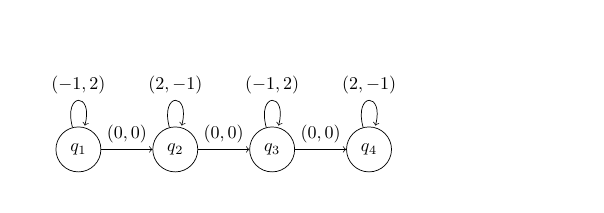
\begin{tikzpicture}[scale=0.25]
\usetikzlibrary{automata, positioning}
\scalebox{0.65}{
\node[state] (q1) {$q_1$};
\node[state, right=of q1] (q2) {$q_2$};
\node[state, right=of q2] (q3) {$q_3$};
\node[state, right=of q3] (q4) {$q_4$};

\path[->] (q1) edge [loop above] node[above] {$(-1,2)$} (q1) edge node[above] {$(0,0)$} (q2); 
\path[->] (q2) edge [loop above] node[above] {$(2,-1)$} (q2) edge node[above] {$(0,0)$} (q3);
\path[->] (q3) edge [loop above] node[above] {$(-1,2)$} (q3) edge node[above] {$(0,0)$} (q4);
\path[->] (q4) edge [loop above] node[above] {$(2,-1)$} (q4);
}
\end{tikzpicture}
\end{minipage}
\begin{minipage}{0.32\textwidth}
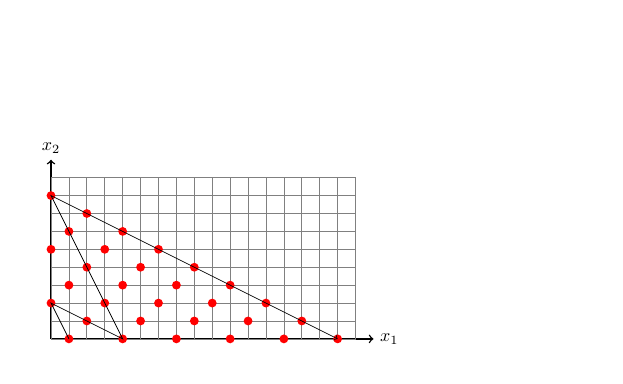
\begin{tikzpicture}[scale=0.35]
\scalebox{0.65}{
\draw[->, thick] (0, 0) -- (18, 0) node[right] {$x_1$};
\draw[->, thick] (0, 0) -- (0, 10) node[above] {$x_2$};

\draw[step=1, gray, thin] (0, 0) grid (17, 9);

\foreach \x in {1,4,7,10,13,16} \fill[red] (\x,0) circle (7pt);
\foreach \x in {2,5,8,11,14} \fill[red] (\x,1) circle (7pt);
\foreach \x in {0,3,6,9,12} \fill[red] (\x,2) circle (7pt);
\foreach \x in {1,4,7,10} \fill[red] (\x,3) circle (7pt);
\foreach \x in {2,5,8} \fill[red] (\x,4) circle (7pt);
\foreach \x in {0,3,6} \fill[red] (\x,5) circle (7pt);
\foreach \x in {1,4} \fill[red] (\x,6) circle (7pt);
\foreach \x in {2} \fill[red] (\x,7) circle (7pt);
\foreach \x in {0} \fill[red] (\x,8) circle (7pt);

\draw[->] (1,0) -- (0,2) -- (2,1) -- (4,0) -- (3,2) -- (2,4) -- (1,6) -- (0,8) -- (2,7) -- (4,6) -- (6,5) -- (8,4) -- (10,3) -- (12,2) -- (14,1) -- (16,0);
}
\end{tikzpicture}
\end{minipage}
\begin{minipage}{0.32\textwidth}
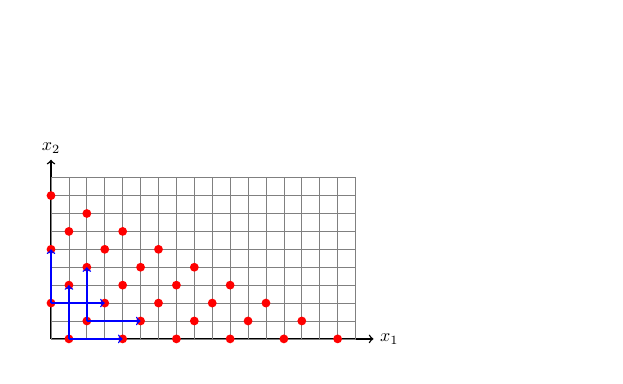
\begin{tikzpicture}[scale=0.35]
\scalebox{0.65}{
\draw[->, thick] (0, 0) -- (18, 0) node[right] {$x_1$};
\draw[->, thick] (0, 0) -- (0, 10) node[above] {$x_2$};

\draw[step=1, gray, thin] (0, 0) grid (17, 9);

\foreach \x in {1,4,7,10,13,16} \fill[red] (\x,0) circle (7pt);
\foreach \x in {2,5,8,11,14} \fill[red] (\x,1) circle (7pt);
\foreach \x in {0,3,6,9,12} \fill[red] (\x,2) circle (7pt);
\foreach \x in {1,4,7,10} \fill[red] (\x,3) circle (7pt);
\foreach \x in {2,5,8} \fill[red] (\x,4) circle (7pt);
\foreach \x in {0,3,6} \fill[red] (\x,5) circle (7pt);
\foreach \x in {1,4} \fill[red] (\x,6) circle (7pt);
\foreach \x in {2} \fill[red] (\x,7) circle (7pt);
\foreach \x in {0} \fill[red] (\x,8) circle (7pt);

\draw[->,blue,thick] (1,0) -- (4,0);
\draw[->,blue,thick] (1,0) -- (1,3);

\draw[->,blue,thick] (2,1) -- (5,1);
\draw[->,blue,thick] (2,1) -- (2,4);

\draw[->,blue,thick] (0,2) -- (3,2);
\draw[->,blue,thick] (0,2) -- (0,5);
}
\end{tikzpicture}
\end{minipage}
\caption{Left: 4-component \dvass $V_2$. 
Middle: the set $\reach_{q_4}(V_2, q_1(1,0))$ and a path $q_1(1,0) \tran q_4(16,0)$.
Right: bases 
%$A = \{(1,0),(2,1),(0,2)\}$ 
and periods 
%$P = \{(0,3),(3,0)\}$
 of an over-approximating semi-linear set $A+P^*$.}
\label{fig:zigzag}
\end{figure}

\begin{example}
For $k\geq 1$, let $V_k$ be a $(2k)$-component \dvass, where each component has just one state $q_i$
and one transition:
$(q_i, (-1,2), q_i)$ for odd $i$, and $(q_i, (2,-1), q_i)$ for even $i$.
Bridge transitions are $(q_i, (0,0), q_{i+1})$.
Figure~\ref{fig:zigzag} shows $V_2$ (left) and 
a path in $V_2$ from $s = q_1(1,0)$ to $t = q_4(16,0)$ together with 
the reachability set $\reach_{q_4}(V_2, s)$ (middle).
In general,
\begin{align} \label{eq:reachk}
X_k := \reach_{q_{2k}}(V_k, s) \ = \ \set{(x_1,x_2) \mid x_1+2x_2 \leq 4^k, \  x_1+2x_2 \equiv 1 \!\! \mod 3}.
\end{align}
Even if the size of the reachability set is 
exponential in $k$, for small $(x_1, x_2)$ it is periodic and the periods are small.
The set $X_k$ can be over-approximated by $A + P^*$ for $A = \set{(1,0),(2,1),(0,2)}$ and $P = \set{(0,3),(3,0)}$
(shown on the right of Figure~\ref{fig:zigzag}), namely for every $k\geq 1$ and $B\in\N$,
the set $X_k$ is \kanapka {$8$} {$B$}. 
For illustration, consider $Y := X_k \cap ((1,0) + P^*)$.
If $(1,0) + P^{\leq B} \subseteq X_k$ then $Y$ is a $B$-approximation
of $(1,0) + P^*$ with $\norm((1,0)), \norm(P) \leq 3 \leq 8$. 
Otherwise, there is some $(v_1, v_2) \in \big((1,0) + P^{\leq B}\big)\setminus X_k$, and
then $B$ is larger than $4^k$:
\[
%8B \geq 2(1 + 3B) \geq 2(v_1 + v_2) \geq v_1 + 2 v_2 > 
4^k < v_1 + 2 v_2 \leq 2(v_1 + v_2) \leq 2(1+3B) \leq 8B.
\]
Therefore by \eqref{eq:reachk}, each $(x_1,x_2) \in Y$ satisfies 
$\norm(x_1,x_2) = x_1 + x_2 \leq x_1 + 2x_2 \leq 4^k < 8B$, and thus
$Y$, seen as a union of singletons, is a union of 
linear sets with norm of base bounded by $8B$ and empty set of periods. 
In both cases, 
$Y$ is \kanapka {$8$} {$B$}. 
%The same intuition stays behind polynomial approximability of \dvass stated in Lemma~\ref{lem:2vass-sandwich}.
\end{example}

% \section{Lessons Learned and Community Impact}
% \label{sec:lessons}
% \section{Practical Lessons}
\label{sec:lessons}

This section shares the practical lessons we learn during developing and optimizing the performance of \modelname. Note that the numbers in this section are not evaluated on the latest benchmarks, thus may be inconsistent with those in previous sections.

%\subsection{Balancing Fine-tuning Data}
\stitle{Balancing fine-tuning data}
We use full parameter fine-tuning to speedup model adaption and we find that the distribution of evaluation scores and pairwise ratings of fine-tuning data severely influences the rating bias of the obtained model. For instance, we fine-tuned an earlier version of \modelname with all single answer grading evaluation records, and the resulting MAE and \agrpq{2}{2} are 1.068 and 0.455 on the \aligndata benchmark, much worse than its teacher GPT-4 with 0.868 and 0.509. During model diagnosis we observe that the model has an extreme high trend to rate response with score 4. We check the distribution of scores in the fine-tuning data and find that evaluation records with score 4 account for approximately 56\%. We then down-sample these records to achieve a more balanced score distribution, leading to optimized MAE and \agrpq{2}{2} with 0.908 and 0.467. And the predicted scores are less biased to a specific one.




%\subsection{Supporting Custom Evaluation Prompts}
\stitle{Supporting custom evaluation prompts}
Recall Table~\ref{tab:prompt} that our scenario-based prompts use fixed criteria, steps, and a five-tier rating system for evaluation. During the deployment of \modelname, our initial users request for supporting custom prompts for criteria and rating systems. To this end, we have constructed a custom prompt generation procedure which augments required data without extra API usage for GPT-4.


% As shown in Appendix~\ref{app:scenario} and , each scenario is designed with a fixed number of criteria, and the scoring ranges from 1 to 5. To meet the personalized needs of users, such as customized criteria names and descriptions, number of criteria, and score ranges, we have constructed a custom prompt process through the following steps.

\etitle{(1) Rephrasing criteria and descriptions}
Referring to~\cite{Ovadia2023FTorRAG}, we employ an LLM to paraphrase existing criteria, requiring the paraphrased names and descriptions to have low textual similarity to the original, while maintaining semantic consistency. After manual check the results, we obtain over 2,400 name-description pairs as complement to the original ones. We then replace the original criteria with the corresponding rephrased ones.
%To ensure consistency between input and output, the criteria name in the output are replaced with the corresponding paraphase results.

\etitle{(2) Diversifying effective criteria in evaluations}
To accommodate possibly various user-defined criteria, we employ a random sampling strategy of  effective criteria in each evaluation to enhance the generalization of our model. Note that \modelname performs evaluation by firstly assigning scores for each criterion and then aggregating these scores to derive a final score. Consequently, criteria down-sampling necessitates recalculation of the final scores.
% 
To achieve this, we have developed a method wherein we extract scores from existing evaluation records. We then train a regression model to predict the final score from each criteria grade. Results show that such a simple regression model achieves a MAE of only 0.12 evaluated on a reserved validation set. %, indicating that the regression model meets the usability standards.
Subsequently, we derive extra evaluation records by down-sampling effective criteria and updating the final scores with the regressed.
%we first categorize the criteria for each sample into relevant and irrelevant. Criteria deemed irrelevant either receive no score or are marked as "Not Applicable" in our outputs. We employ a random sampling probability between 0.5 and 1 to select these two groups of criteria. We then substitute the original input and output data with the down-sampled criteria and the recalculated final scores.

\etitle{(3) Using alternative rating systems}
Except for the 5-tier rating, other systems are also popular for evaluation, such as binary (0-1 or 1-2), 3-class (1-3), and 10-class (1-10) ratings. To accommodate them, we transform the original scores into other systems with heuristic score mapping rules.
% redirected the 5 classes. For binary classification, scores of 1-3 are grouped into the first category, and 4-5 into the second category; for 3-class, scores of 1-2, 3, and 4-5 are divided into different categories; for 10-class, we multiply the scores by 2 and minus 1 to the doubled score with a 50\% probability.


\etitle{(4) Hybrid customization} 
To achieve optimal model performance, we mixed the aforementioned operations in different proportions, resulting in our final augmented fine-tuning data.


While supporting custom evaluation prompts is initially a functional requirements, we also observe improvement on performance: the MAE exhibited reductions from (0.699, 0.703) to (0.684, 0.676) and the \agrpq{2}{2} are improved from (0.577, 0.569) to (0.586, 0.581)
% and \agrpq{2}{2} are improved from (0.699, 0.577) and (0.703, 0.569) to (0.684, 0.586) and (0.676, 0.581) 
on the two benchmarks, respectively. Research on learning theory of LLMs provides a plausible explanation for the improvement. Note that fixed prompts lead to duplicated fine-tuning data, which will strengthen the memorization effect while weakening the generalization ability of LLMs~\cite{llm-acquire-know}. Custom evaluation prompts could be regarded as a de-duplication step, enhancing the generalization of the resulting models.
Similarly, we also observe the improvement by using a large batch size. 


\begin{figure}[t]
    \centering
    \includegraphics[width=0.95\linewidth]{images/loss_v2.pdf}
    \caption{Our multi-objective training method.}
    \label{fig:loss}
\end{figure}


%\subsection{Enabling Multi-objective Training}
\stitle{Enabling multi-objective training}
In the standard SFT process, LLMs learn from predicting the exact next tokens by minimizing the cross entropy loss.
However, we note that not all tokens in the evaluation output need to be ``perfectly" predicted. 
Take the output in Fig~\ref{fig:loss} as an example. The content in black is scores and format-related text, and  we require these words to be predicted accurately. On the other hand, the words in blue are the explanation for the specific score, for which we could tolerate more noises as long as the predicted content is semantically similar to the target.


This idea inspires a multi-objective training method illustrated in Fig~\ref{fig:loss}. Specifically, we first label each output tokens with either SFT or Sim. For SFT tokens, we still minimize the cross entropy loss between the the predicted and ground-truth logits. For Sim tokens, we minimize the difference between the embeddings of the top-1 predicted and ground-truth tokens. We find that this training method reduces the 
MAE from (0.684, 0.676) to (0.673, 0.652) and improves \agrpq{2}{2} from (0.586, 0.581) to (0.594, 0.591)
% performance by (0.684, 0.586) and (0.676, 0.581) to (0.673, 0.594) and (0.652, 0.591) 
on the two benchmarks, respectively.



%Firstly, we utilize regular expressions to separate the format-and-score words from the reasons and then employ the tokenizer to return the corresponding word-token mapping. Then a loss mask is generated to indicate which tokens should be associated with the CEL and which should be associated with the Similarity Loss. To transform the logits of shape 'vocabulary-size' into embedding shape, we directly applied matrix multiplication between the logits and the word-embedding layer to obtain the corresponding output embeddings. The similarity between the output embeddings and the input embeddings is then computed using either L2 loss or cosine similarity. At the stage of training, we compute both the CEL and Similarity Loss for all tokens, and combine these two losses to obtain the final training loss with the loss mask.

%\subsection{Unifying Performance Metrics}
\stitle{Unifying performance metrics}
We finally share a lesson for development efficiency. During our deployment of \modelname, a long-term challenge is to determine which fine-tuned checkpoint, or equivalently the corresponding optimization technique, is better. Recall that \modelname supports three variants of evaluations, which is a tradition for the LLM-as-a-Judge paradigm, as well as we create two benchmarks and use two metrics for performance assessment. Putting these together, we need to compare more than 10 numbers to come to a decision, which is not easy. Indeed, we have had a lot of controversies for which one is better within our team. Later, we decide to aggregate all performance metrics into one to close controversies. The most straightforward method is to use the average score. However, we find this is unfair due to the different effective scales for metrics. For instance, it is much harder to optimize the \agrpq{2}{2} by 0.1 than MAE. In this case, using average score will let MAE dominate the choice of optimization directions. 
To address this, we perform a linear transformation on the original metrics such that random guessing is mapped to 0 and the best performance metric is mapped to 1. Averaging the  transformed metrics gives us a fair overall performance metric which help us choose promising optimization strategies.



\section{Reflections and Lessons Learned}
\label{sec:lessons}
The design and implementation of \jjodel{} provided invaluable insights into the challenges and opportunities of creating a modern and user-friendly modeling platform. These lessons, which span architectural decisions, usability considerations, and technology integration, offer a foundation for advancing the field of MDE tools while reflecting on the successes and setbacks encountered during platform development.

\subsection{The Impact of Technology Choices}

The selection of foundational technologies such as Node.js and React played a key role in shaping the architecture, scalability, and usability of \jjodel{}. Node.js introduced a lightweight event-driven back-end optimized for real-time interactions, providing the performance and responsiveness necessary for a collaborative modeling platform. React’s component-based architecture (not to be confused with that of the EMF ecosystem)  enabled modularity and reusability, allowing dynamic syntax customization and intuitive user interface design. However, adopting these frameworks was not straightforward; it required a significant paradigm change in application development and iterative testing to align their architectural models with the goals of \jjodel{}.

The broader evolution of the full-stack web ecosystem underscores the growing influence of these technologies. Key advancements such as Node.js (2009), Angular.js (2010), React (2013), and Vue.js (2014) have transformed the way modern applications are designed and developed. By 2024, Node.js powers over 40\% of web applications, cementing its role as a preferred backend technology in low-code platforms. React, used by 39.5\% of front-end developers, integrates seamlessly with advanced interfaces, making it a leading choice for creating responsive, component-based UIs\footnote{\url{https://www.statista.com/statistics/1124699/worldwide-developer-survey-most-used-frameworks-web/?utm_source=chatgpt.com}, last accessed on January 9, 2025}. These frameworks highlight the stark contrast in user experience between traditional modeling tools (all first released before), often emphasizing technical rigor, and modern low-code development platforms (LCDPs)~\cite{sahay2020supporting,prinz2021low}, which prioritize usability, real-time collaboration, and seamless adaptability.

For \jjodel{}, the decision to adopt Node.js and React was driven by the need to balance accessibility, flexibility, and \textit{richness}—qualities often absent in traditional tools. Node.js provided the foundation for real-time interactions, while React’s modular architecture empowered the platform to deliver an intuitive and customizable user experience. Together, these technologies helped \jjodel{} align its design with the broader goals of scalability and usability, ensuring that the platform could meet the diverse needs of its users. This process underscored the importance of carefully integrating technological frameworks to shape not only the technical implementation but also the overall user experience.

Crucially, these insights were not evident at the beginning. They emerged through a process of trial and error, with one particularly challenging iteration spanning two years of development. This iterative approach, guided by the expertise and advocacy of one of the authors, ultimately enabled the team to make informed decisions and implement a modern, scalable architecture for \jjodel{}.

In summary, the development of \jjodel{} reinforced a critical realization: technology is not neutral. It defines both the possibilities and constraints of a platform, influencing its ability to innovate and its inherent limitations. 
%These lessons highlight the pivotal role of thoughtful technology choices in ensuring that platforms align with their goals and fulfill their potential.

\subsection{Balancing Flexibility and Simplicity}
Balancing the flexibility of the platform with its usability proved to be one of the most significant challenges in the development of \jjodel{}. Many features were essential to meeting the requirements we add in mind~\cite{di2023jjodel}, but their integration risked introducing unnecessary complexity. To address this, \jjodel{} adopted a progressive disclosure approach, where essential features were initially exposed and advanced functionalities could be revealed later. Like this, both novice and experienced users could interact with the platform more effectively.

The decision to prioritize simplicity without compromising flexibility was further informed by user feedback. Iterative testing demonstrated that users, particularly those new to MDE tools, found overwhelming interfaces to be a barrier to productivity. By simplifying initial interactions and allowing users to explore more advanced features, \jjodel{} demonstrated that even complex modeling platforms could cater to diverse audiences while retaining powerful capabilities. 

\subsection{Avoiding Accidental Complexity}

Reducing accidental complexity~\cite{atkinson2008reducing} was a cornerstone of the \jjodel{} project. Traditional MDE tools often require complex installation procedures and specialized technical expertise, which hinder accessibility for students and domain experts. By prioritizing a client-side intelligence model, \jjodel{} eliminated many of these barriers, enabling users to engage with the platform without requiring advanced setup or configuration.

This decision significantly improved the accessibility and usability of the platform, aligning with its mission to democratize modeling practices. In addition, the streamlined architecture and processes reduced the cognitive load for users, allowing them to focus on their tasks rather than the intricacies of the tool itself. This approach highlights the importance of designing platforms that prioritize usability without sacrificing flexibility or power.

\subsection{Rethinking Concrete Syntax}

The integration of React’s component-based architecture into \jjodel{} fundamentally transformed how concrete syntax was conceptualized and rendered. Unlike traditional modeling tools, which often rely on static and rigid representations, the proposed approach allowed dynamic customization and real-time interaction. This flexibility enabled users to define syntax viewpoints tailored to their specific needs, fostering a more intuitive modeling experience.

This innovation also demonstrated the potential of modern web technologies to drive advancements in traditionally static domains. Using React's state management and rendering capabilities, \jjodel{} bridged the gap between abstract modeling concepts and practical applications, providing users with a seamless and interactive experience.

\subsection{Iterative Design and Feedback}

The iterative development process~\cite{4668134} was central to the success of \jjodel{}. Regular testing with novice and experienced modelers revealed critical gaps in usability and functionality, informing refinements in interface design and platform features. Early feedback emphasized the importance of real-time feedback mechanisms and context-aware interfaces, leading to the implementation of progressive disclosure and other user-centric design principles.

This approach ensured that \jjodel{} evolved as a responsive and adaptive platform, capable of meeting the diverse needs of its user base. The iterative process also reinforced the value of engaging with stakeholders throughout development, ensuring that the platform remained aligned with user expectations and requirements.

\subsection{Navigating Trade-offs}

Departing from established standards, such as Eclipse GLSP~\cite{bork2023vision}, presented significant challenges and unique opportunities for \jjodel{}. This decision enabled the platform to align more closely with its meta-metamodel, a strict extension of Ecore, and to prioritize client-side intelligence. IAlthough it resulted in a less standardized architecture, the trade-off proved advantageous, making the platform more reactive and agile while eliminating cumbersome integration processes often associated with traditional frameworks.

This experience highlights the critical importance of carefully evaluating trade-offs in platform design. By prioritizing flexibility and usability over strict adherence to established frameworks, we took a calculated risk that ultimately paid off. The resulting architecture demonstrated that divergence from canonical approaches, when guided by clear objectives, can lead to innovative and effective solutions aligned with the vision and goals of the platform.

\subsection{Exploring Alternatives to OCL.js}
Our experience with OCL.js\footnote{\url{https://ocl.stekoe.de/}}, a JavaScript-based implementation of the Object Constraint Language (OCL), provided both opportunities and challenges during the development of \jjodel{}. Despite OCL.js offered full integration with \jjodel{} and initially appeared to be a natural fit, its limitations became apparent over time. The lack of active development of the project and its partial coverage of the OCL standard forced us to explore alternatives to define constraints and predicates within the platform.

The most natural alternative was to adopt the declarative and functional expressions of JSX, which \jjodel{} already uses to template. This approach allowed us to leverage the same notation for both templating and predicates, creating a consistent and simplified user experience. However, it also introduced new uncertainties. To the best of our knowledge, JSX has not been formally characterized and no direct comparison between JSX and OCL has been documented in the literature. This absence of formalization leaves open questions about the expressive power, correctness, and potential limitations of JSX as a substitute for OCL.

This experience underscores the importance of evaluating the trade-offs between adopting emerging notation like JSX and relying on established but limited standards like OCL.js. Although JSX has served \jjodel{} well in the short term, further research and validation is necessary to determine its suitability as a foundational element to define constraints and predicates.

\subsection{The Value of Learning Through Failure}

Some of the most valuable lessons emerged from the failures encountered during development. Iterative attempts to align the architectural design with the objectives of the platform revealed the complexity of creating a scalable, reactive system~\cite{lyytinen1999learning}. In one instance, a two-year iteration led to significant revisions, demonstrating the importance of persistence and openness in addressing setbacks.

This experience reinforced the value of accepting failure as an opportunity for growth. Learning from missteps, \jjodel{} was able to refine its approach and develop a platform that is both innovative and user-friendly. The development of \jjodel{} underscored the importance of balancing technical innovation with user-centric design. The lessons learned highlight the need for thoughtful technology choices, iterative development, and a willingness to embrace trade-offs and failures as opportunities for growth. These insights provide a foundation for advancing the field of MDE tools, ensuring that future platforms are both powerful and accessible.

\section{Related Work}
\label{sec:rw}
This section reviews various MDE platforms, discussing their features, strengths, and limitations to position \jjodel{} within the current landscape of MDE tools.

MetaEdit+ \cite{Kelly2013} is a mature and widely recognized platform for domain-specific modeling (DSM). It uses the GOPPRR meta-metamodeling language \cite{kelly2005domain} to define domain-specific concepts and relationships, offering extensive customization capabilities. Despite its introduction in 1995 and its reliance on an outdated technology stack, MetaEdit+ features a reflective and integrated architecture that provides robust operational support through built-in governance mechanisms. These capabilities simplify complex tasks, such as ensuring metamodel consistency and managing artifacts, challenges that remain prevalent in many other MDE tools.
%
In comparison, \jjodel{} inherits the strengths of MetaEdit +, such as its reflective and integrated architecture. Leveraging a native cloud architecture and cutting-edge front-end technologies, \jjodel{} offers a more \textit{transparent} user experience by minimizing the accidental complexity, alongside support for real-time collaboration and automated syntax co-evolution. 
%These features make \jjodel{} particularly well-suited for agile, iterative, and distributed development workflows.

GMF/Eugenia\footnote{\url{https://eclipse.dev/modeling/gmp/}}, built on the Eclipse Modeling Framework (EMF), facilitates the automated generation of graphical editors. These tools are powerful in defining graphical representations. Unfortunately, their dependence on intricate configurations and technical complexity poses significant challenges for non-expert users. Moreover, their generative approach and component-based architecture hinder their ability to support dynamic adaptability, an essential feature for iterative and agile development workflows, as well as real-time collaboration. In contrast, \jjodel{} overcomes these limitations with an intuitive low-code environment that combines dynamic syntax customization with seamless collaboration, making it a more practical and efficient choice for modern team-based modeling scenarios.

Sirius\footnote{\url{https://eclipse.dev/sirius/}}, also built on the Eclipse ecosystem, introduces viewpoint-based modeling, allowing users to define and work with multiple perspectives in a single model. While this approach reduces programming effort, Sirius remains configuration-intensive and lacks native support for real-time collaboration or dynamic syntax co-evolution, limiting its adaptability in iterative and distributed development workflows. In contrast, the reflective architecture of \jjodel{} incorporates built-in governance mechanisms, often absent in tools such as Sirius, that simplify complex tasks such as coevolution and validation of metamodels, providing a more streamlined and robust modeling experience.

Building on the concepts of its predecessor, Sirius Web \cite{Giraudet2024} transitions to a native web environment, using React to deliver a modern interface. It introduces collaborative modeling features and supports various representation types, including diagrams, forms, and Gantt charts. While these advancements address some limitations of Sirius Desktop, Sirius Web still suffers from significant configuration overhead and limited dynamic adaptability, which constrain its effectiveness in highly iterative and fast-paced projects. Furthermore, its component-based architecture, rooted in EMF, lacks the seamless integration of an all-in-one environment, leading to fragmentation and increased complexity for users. 
%In contrast, \jjodel{} offers a fully declarative and reflective architecture, improving usability and governance while simplifying complex modeling tasks, such as metamodel co-evolution. By providing a seamlessly integrated environment, \jjodel{} ensures greater agility and adaptability to rapidly changing requirements, making it particularly well-suited for collaborative and dynamic modeling scenarios.

Sprotty\footnote{\url{https://sprotty.org/}} and Gentleman \cite{3417990.3421998} address narrower roles in the MDE ecosystem. Sprotty is a web-based visualization framework focused on rendering lightweight models, while Gentleman provides a flexible projectional editing interface for directly modifying abstract syntax trees. Although these tools excel in specific use cases, they lack deeper integration with metamodel evolution and collaboration workflows. \jjodel{} combines the simplicity and lightweight design of tools like Sprotty and Gentleman with advanced capabilities such as automated syntax co-evolution, making it a more comprehensive solution.


A recent paper by Metin et al.~\cite{Metin2025} explores the challenges and lessons learned from working with GLSP and developing several GLSP-based modeling tools. The authors present a reusable reference architecture designed to facilitate the development and operation of GLSP-based web modeling tools. The reference architecture is then instantiated using BigUML as a running example. The paper highlights the procedural approach, key lessons learned, and critical reflections on the challenges and opportunities associated with using GLSP. In contrast to \jjodel{}, which natively supports cloud-based modeling, GLSP-based web modeling tools require the ad hoc implementation of the domain language, adding an additional layer of complexity.

HyperGraphOS \cite{Ceravola2024} represents an ambitious vision, integrating DSLs, modeling, and task execution into a unified system. Its infinite workspace concept and AI-enhanced adaptability demonstrate significant innovation, but these features come at the expense of usability for less technical users. 
%In contrast, \jjodel{} offers a more balanced approach, focusing on accessibility and iterative workflows, making it ideal for teams that prioritize usability and collaboration over extensive technical features.

Many of the platforms surveyed possess industrial-grade or commercial-technology readiness levels (TRL), making them well suited for high-stakes, large-scale projects. In contrast, \jjodel{} remains an academic endeavor, designed to explore and adapt the principles and solutions commonly found in large-budget projects and low-code platforms. Translating these into accessible and innovative approaches, \jjodel{} makes a unique contribution to the field. However, this academic focus also highlights its limitations in directly competing with fully commercialized solutions, particularly in terms of scalability, robustness, and enterprise-level support.
%
However, the initial adoption of \jjodel{} in academic settings has yielded promising results. Although a systematic evaluation of its impact on teaching and learning outcomes has not yet been conducted, preliminary feedback has been highly encouraging. Students have demonstrated significant engagement and understanding, even in the absence of extensive learning resources at the time of the course\footnote{For more details on the survey results, see \url{https://www.jjodel.io/student-survey/}.}. These early findings indicate that \jjodel{} has the potential to become a valuable educational tool, particularly in model-driven engineering courses.

\section{Conclusions and Future Work}
\label{sec:conclusion}
\section{Conclusion}
In this work, we propose a simple yet effective approach, called SMILE, for graph few-shot learning with fewer tasks. Specifically, we introduce a novel dual-level mixup strategy, including within-task and across-task mixup, for enriching the diversity of nodes within each task and the diversity of tasks. Also, we incorporate the degree-based prior information to learn expressive node embeddings. Theoretically, we prove that SMILE effectively enhances the model's generalization performance. Empirically, we conduct extensive experiments on multiple benchmarks and the results suggest that SMILE significantly outperforms other baselines, including both in-domain and cross-domain few-shot settings.

\bibliographystyle{abbrv}  
\bibliography{bib.bib}   






\end{document}
% end of file template.tex

